\documentclass[11pt]{article}
\usepackage[a4paper,margin=2.2cm]{geometry}
\usepackage[utf8]{inputenc}
\usepackage[T1]{fontenc}
\usepackage{tikz}
\usetikzlibrary{arrows.meta,positioning,shapes.geometric}
\usepackage{booktabs}
\usepackage{longtable}
\usepackage{array}
\usepackage{enumitem}
\usepackage{titlesec}
\usepackage{hyperref}

\titleformat{\section}{\large\bfseries}{P\arabic{section}.}{0.5em}{}
\titlespacing{\section}{0pt}{1.2em}{0.6em}

\title{\textbf{Prueba Práctica --- Unidad IV\\ Ingeniería de Requisitos (ISR-401)}\\
\large Caso: Sistema de Gestión de Pedidos}
\author{Anthony Alfredo Vera Gómez}
\date{Universidad Técnica Estatal de Quevedo\\ Facultad de Ciencias de la Ingeniería --- Carrera de Ingeniería de Software}

\begin{document}
\maketitle

\section{Modelo de datos --- Diagrama de clases UML}

\begin{center}
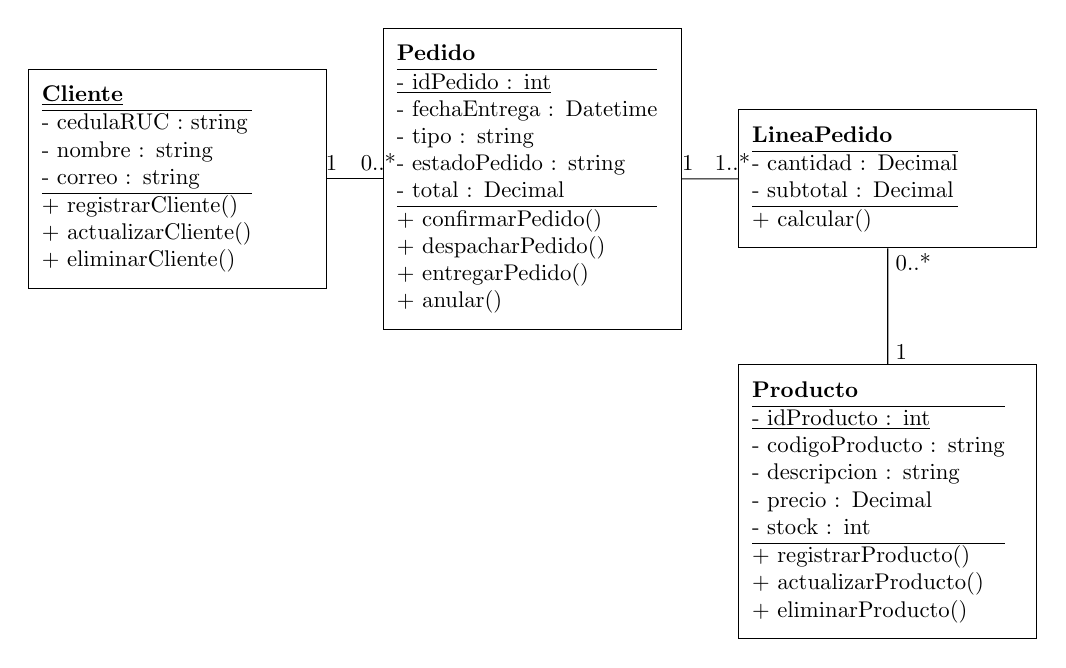
\begin{tikzpicture}[
  class/.style={rectangle, draw, align=left, text width=4.2cm, inner sep=6pt},
  >=Stealth, scale=0.82, every node/.append style={scale=0.82}
]

\node[class] (cliente) at (0,0) {
  \begin{tabular}[t]{@{}l@{}}
  \underline{\textbf{Cliente}}\\ \hline
  - cedulaRUC : string\\
  - nombre : string\\
  - correo : string\\ \hline
  + registrarCliente()\\
  + actualizarCliente()\\
  + eliminarCliente()
  \end{tabular}
};

\node[class] (pedido) at (5.5,0) {
  \begin{tabular}[t]{@{}l@{}}
  \textbf{Pedido}\\ \hline
  \underline{- idPedido : int}\\
  - fechaEntrega : Datetime\\
  - tipo : string\\
  - estadoPedido : string\\
  - total : Decimal\\ \hline
  + confirmarPedido()\\
  + despacharPedido()\\
  + entregarPedido()\\
  + anular()
  \end{tabular}
};

\node[class] (linea) at (11,0) {
  \begin{tabular}[t]{@{}l@{}}
  \textbf{LineaPedido}\\ \hline
  - cantidad : Decimal\\
  - subtotal : Decimal\\ \hline
  + calcular()
  \end{tabular}
};

\node[class] (producto) at (11,-5) {
  \begin{tabular}[t]{@{}l@{}}
  \textbf{Producto}\\ \hline
  \underline{- idProducto : int}\\
  - codigoProducto : string\\
  - descripcion : string\\
  - precio : Decimal\\
  - stock : int\\ \hline
  + registrarProducto()\\
  + actualizarProducto()\\
  + eliminarProducto()
  \end{tabular}
};

\draw (cliente) -- (pedido)
  node[pos=0.08, above] {1} node[pos=0.92, above] {0..*};
\draw (pedido) -- (linea)
  node[pos=0.1, above] {1} node[pos=0.9, above] {1..*};
\draw (linea) -- (producto)
  node[pos=0.12, right] {0..*} node[pos=0.9, right] {1};

\end{tikzpicture}
\end{center}

\section{Modelo funcional --- Diagrama de actividades UML}
\textit{Proceso: Registrar Pedido}

\begin{center}
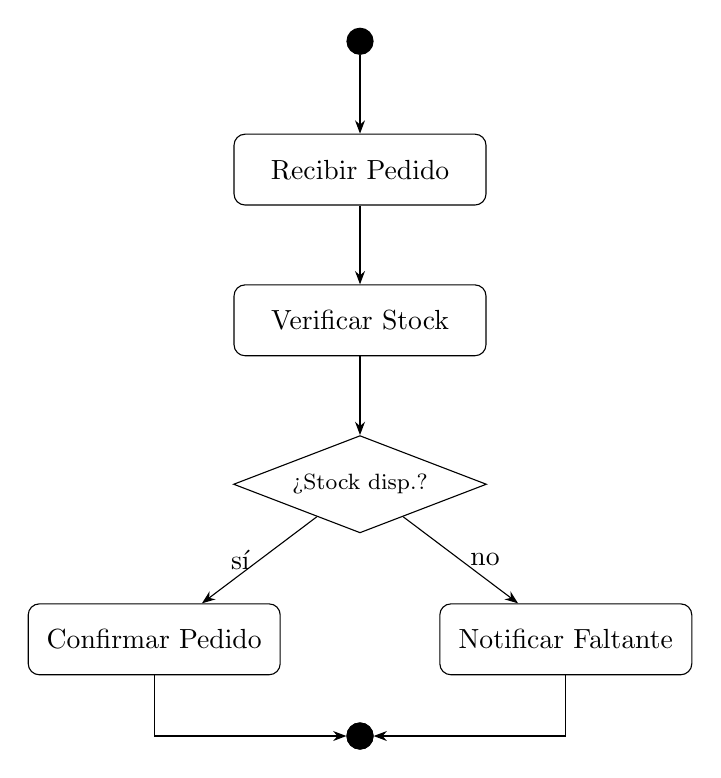
\begin{tikzpicture}[
  act/.style={rectangle, draw, rounded corners, align=center, minimum width=3.2cm, minimum height=0.9cm},
  node distance=1cm and 1cm,
  >=Stealth
]
\node[circle, draw, fill=black, minimum size=6pt] (start) {};
\node[act, below=of start] (recibir) {Recibir Pedido};
\node[act, below=of recibir] (verificar) {Verificar Stock};
\node[diamond, draw, aspect=2.6, below=of verificar, minimum width=2.6cm, font=\footnotesize] (decision) {¿Stock disp.?};
\node[act, below left=1.2cm and 0.2cm of decision] (confirmar) {Confirmar Pedido};
\node[act, below right=1.2cm and 0.2cm of decision] (notificar) {Notificar Faltante};
\node[circle, draw, fill=black, minimum size=6pt, below=2.4cm of decision] (end) {};
\node[circle, draw, minimum size=8pt] at (end) {};

\draw[->] (start) -- (recibir);
\draw[->] (recibir) -- (verificar);
\draw[->] (verificar) -- (decision);
\draw[->] (decision) -- node[left] {sí} (confirmar);
\draw[->] (decision) -- node[right] {no} (notificar);
\draw[->] (confirmar) |- (end);
\draw[->] (notificar) |- (end);
\end{tikzpicture}
\end{center}

\section{Máquina de estados UML}


\section{Consistencia entre las tres perspectivas}

\begin{center}
\begin{tabular}{@{}llll@{}}
\toprule
\textbf{Evento (P3)} & \textbf{Función (P2)} & \textbf{Entidad/Atributo (P1)} \\
\midrule
Confirmar & confirma el pedido & Pedido.estadoPedido \\
Despachar & despacha el pedido & Pedido.estadoPedido \\
Entregar  & entrega el pedido  & Pedido.estadoPedido \\
Anular    & anula el pedido    & Pedido.estadoPedido \\
\bottomrule
\end{tabular}
\end{center}

\textbf{Inconsistencia detectada:} el diagrama de actividades (P2) modela únicamente el subproceso
``Registrar Pedido'' (recibir $\rightarrow$ verificar stock $\rightarrow$ confirmar/notificar), pero no
representa las acciones \texttt{despachar}, \texttt{entregar} ni \texttt{anular} que sí aparecen en la
máquina de estados (P3). Existen eventos sin función modelada explícitamente en P2.
\textbf{Corrección:} se debe ampliar el diagrama de actividades con un segundo flujo ``Gestionar ciclo
de vida del pedido'' que incluya las actividades Despachar Pedido, Entregar Pedido y Anular Pedido,
manteniendo la coherencia con los estados de P3.

\section{Especificación de requisitos con esquema de atributos}

\begin{itemize}[leftmargin=1.6cm]
\item[\textbf{RF-01}] El sistema debe registrar un pedido con sus líneas y productos.
\item[\textbf{RF-02}] El sistema debe verificar el stock antes de confirmar una entrega.
\item[\textbf{RNF-01}] El sistema debe proteger los datos del cliente \textit{(Seguridad --- ISO/IEC 25010)}.
\item[\textbf{RNF-02}] El sistema debe registrar los pedidos con rapidez, en menos de 3 segundos \textit{(Eficiencia de desempeño --- ISO/IEC 25010)}.
\end{itemize}

\begin{center}
\small
\begin{tabular}{@{}lllllll@{}}
\toprule
\textbf{ID} & \textbf{Prioridad} & \textbf{Estado} & \textbf{Fuente} & \textbf{Estabilidad} & \textbf{Versión} & \textbf{Verificación} \\
\midrule
RF-01  & Alta  & Propuesto  & Caso de negocio & Alta  & 1.0 & Prueba \\
RF-02  & Alta  & Propuesto  & Caso de negocio & Alta  & 1.0 & Prueba \\
RNF-01 & Media & Propuesto  & Caso de negocio & Media & 1.0 & Inspección \\
RNF-02 & Media & Propuesto  & Caso de negocio & Media & 1.0 & Prueba de carga \\
\bottomrule
\end{tabular}
\end{center}

\section{Priorización MoSCoW}

\begin{center}
\begin{tabular}{@{}llp{8.5cm}@{}}
\toprule
\textbf{Requisito} & \textbf{Categoría} & \textbf{Justificación} \\
\midrule
RF-01  & Must have   & Es la principal funcionalidad del sistema. \\
RF-02  & Must have   & Garantiza la consistencia de la cantidad del inventario. \\
RNF-01 & Could have  & Garantiza la seguridad y la confianza del cliente. \\
RNF-02 & Should have & Mejora la rapidez en el flujo de datos. \\
\bottomrule
\end{tabular}
\end{center}

\section{Validación por inspección (lista de comprobación 29148)}

Propiedades evaluadas, defecto detectado, retrabajo
\section{Pruebas de aceptación trazadas}

\begin{center}
\small
\begin{tabular}{@{}lllll@{}}
\toprule
\textbf{ID} & \textbf{Tipo} & \textbf{Entradas} & \textbf{Criterio de éxito} & \textbf{Traza} \\
\midrule
PA-01 & Funcional     & Pedido con 2 líneas validadas & Total calculado correctamente & RF-01 \\
PA-02 & Funcional     & Verificación de stock          & El sistema notifica el faltante & RF-02 \\
PA-03 & No funcional  & Seguridad al cliente            & Datos ilegibles para terceros & RNF-01 \\
PA-04 & No funcional  & 100 pedidos simultáneos         & Eficacia en el registro de pedidos & RNF-02 \\
\bottomrule
\end{tabular}
\end{center}

\section{Matriz de trazabilidad}

\begin{center}
\small
\begin{tabular}{@{}lllll@{}}
\toprule
\textbf{Requisito} & \textbf{Fuente} & \textbf{Modelo asociado} & \textbf{Prueba} & \textbf{Dependencia} \\
\midrule
RF-01  & Caso de negocio & P1: Cliente / Pedido / LíneaPedido        & PA-01 & --- \\
RF-02  & Caso de negocio & P2: decisión de stock / Producto.stock    & PA-02 & depende de RF-01 \\
RNF-01 & Caso de negocio & P3: transición anular (protección datos)  & PA-03 & --- \\
RNF-02 & Caso de negocio & P2: flujo ``Registrar Pedido''            & PA-04 & depende de RF-01 \\
\bottomrule
\end{tabular}
\end{center}

\textbf{Requisito huérfano:} ninguno; los cuatro requisitos poseen modelo y prueba asociados.
\textbf{Dependencia horizontal:} RF-02 y RNF-02 dependen de RF-01, ya que ambos actúan sobre un
pedido previamente registrado.

\section{Gestión del cambio y línea base}



\end{document}